\documentclass[../main.tex]{subfiles}
\begin{document}

\chapter{Fragestellung}
\label{question}
  Die Wertschöpfung moderner IT-Unternehmen beruht auf dem Angebot von Diensten, die über das Internet den Nutzern zur Verfügung gestellt werden. Die Dienste werden von Anwendungen realisiert, die i.d.R. in Rechenzentren betrieben werden. Der überwiegende Vermögensgegenstand in diesem Modell ist die Software, die in den Rechenzentren produktiv läuft. Der Wert dieser ist direkt abhängig von Eigenschaften wie der Leistung und Sicherheit eines Rechenzentrums.

  Kunden, die ihr Produkt über Rechenzentren anbieten, sind u.\,a. an Sicherheitsfeatures interessiert, die die Sicherheitsziele aus Abschnitt \ref{introSecGoals} sicherstellen. Je nach Anwendungsfall kommt diesen Zielen unterschiedliche Wichtigkeit zu. Die Erfüllung der Sicherheitsziele muss für einen sicheren Betrieb auf Anwendungs-, Virtualisierungs- und Netzwerkebene gegeben sein.

  Die Betreiber von Rechenzentren streben gleichzeitig einen möglichst effizienten Betrieb der Kundensysteme in der eigenen Infrastruktur an. Wie in Kapitel \ref{basics} gezeigt, bietet der Einsatz von Containertechnologien aus Sicht der Leistung, Effizienz sowie administrativen Faktoren, attraktive Eigenschaften für die Betreiber von Rechenzentren. Mit gegebener Hardware lassen sich z.\,B. mit Containertechnologien durchschnittlich mehr Kundenanwendungen realisieren, wie wenn letztere mit der konventionellen Hypervisortechnologie betrieben werden.

  % Die Betreiber von Rechenzentren wiederum müssen diese Nachfrage befriedigen.
  % Dabei streben sie einen möglichst effizienten
  %, wollen gleichzeitig jedoch auch selbst Gewinn machen. Durch den Betrieb von Containern in Rechenzentren kann im Vergleich zu Hypervisorlösungen theoretisch mehr Gewinn geschöpft werden, da sich mit ihnen - bei gleicher Hardware - mehr virtuelle Kapazität realisieren lässt. Die Sicherheit virtueller Instanzen darf im Betrieb von Containern jedoch nicht leiden, um weiterhin den Kundenanforderungen zu entsprechen.

  Mit den außer Frage stehenden Leistungs- und Effizienzvorteilen ist demnach die erste zentrale Frage für Betreiber von Cloud"=Infrastrukturen, inwiefern Sicherheitsfunktionen von Containertechnologien die erforderlichen Sicherheitsziele erfüllen. Diese Fragestellung kann anhand einer konkreten Untersuchung genauer formuliert werden. Die Untersuchung basiert auf der im Rahmen der \acrshort{CISSP}-Zertifizierung in \cite[S.36]{CISSP} vorgestellten Risikoanalyse sowie den Empfehlungen von NIST in \cite[S.23]{nist}. Die Risikoanalyse dient gleichzeitig dazu, Annahmen vorzustellen und Schlussfolgerungen zu ziehen, auf deren Basis die zu betrachtenden Eigenschaften von Docker gegen Ende dieses Kapitels definiert werden.


  \section{Identifikation des Systems}
    Das Systemmodell von hypervisorbasierten Systemen kann nicht verwendet werden, da das Design der Containersysteme stark von Erstgenannten abweicht. Während nach \cite[S.125]{CISSP} virtuelle Maschinen als eigener Sicherheitsmechanismus des Betriebssystems aufgelistet sind, trifft das für die Containersysteme und deren Architektur nicht zu. Andere Sicherheitsfeatures des Hostsystems müssen aktiviert werden, um die Containersicherheit zu erhöhen.

    \begin{figure}[h]
        \centering
        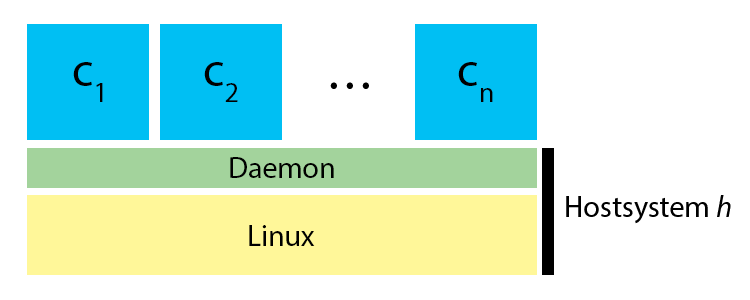
\includegraphics[width=0.8\textwidth]{./images/question_model1.png}
        \caption{Erster Entwurf eines Systemmodells mit Hostsystem und Containern (eigene Abbildung).}
        \label{fig:question_model1}
    \end{figure}

    Das Systemmodell ist zunächst wie in \fig \ref{fig:question_model1} definiert: Es existiert ein Hostsystem \(h\) und eine Containermenge \(M\), die aus den Containern \(c_1,c_2,\dotsc,c_n\) besteht. Die Container werden von einem Docker-Daemon verwaltet, der zusammen mit Linux in \(h\) läuft.

    Verteilte Docker-Systeme, in denen mehrere Hosts miteinander kommunizieren, werden in dieser Arbeit nicht betrachtet. Aus diesem Grund existiert in diesem Systemmodell nur ein Hostsystem \(h\) mit Docker-Installation, das alle Container in \(M\) verwaltet.

  \section{Identifikation der Bedrohungen}
    In diesem Schritt werden die verschiedenen Bedrohungsarten auf Basis des zuvor definierten Systemmodells erörtert.

    Aus \fig \ref{fig:question_model1} und der Funktionsweise von Docker (s. Abschnitt \ref{dockerIntro}) können zwei unterschiedliche Gefahrenquellen (A) und (B) identifiziert werden:

    \begin{enumerate}[label=(\Alph*)]
      \item \textbf{Docker-Spezifika}: In Containern werden Anwendungen ausgeführt, die nicht zwangsweise vertrauenswürdig sind. Wenn beispielsweise Containerimages von einer öffentlichen Registry, wie dem \emph{Docker Hub}, bezogen werden, existiert keine Garantie, dass aus diesen Images gestartete Container nicht gegen die Sicherheitsziele der Vertraulichkeit, Integrität und Verfügbarkeit verstoßen. Durch die Komplexität moderner Anwendungen und deren Abhängigkeiten zu Bibliotheken ist es selbst bei quelloffenen Anwendungen schwierig, diese als vertrauenswürdig einzustufen. Deswegen muss davon ausgegangen werden, dass in Containern willkürliche Programme ablaufen (\emph{interne Gefahrenquellen}), die - versehentlich oder beabsichtigt - den Host schädigen können.

      Außerdem kann jederzeit ein Fehler in der Codebasis von Docker entdeckt werden, der die Sicherheit von Docker"=Hostsystemen und Containern beeinträchtigt.

      \item \textbf{Container als Server im Internet}: Viele Container stellen einen Dienst über das Internet zur Verfügung und stehen dadurch mit der Außenwelt in Kontakt. Ein Webserver beispielsweise kann als Containerapplikation betrieben werden, indem er über einen Port Anfragen von Clients entgegen nimmt und diese nach abgeschlossener Verarbeitung beantwortet. Die Notwendigkeit, Containerschnittstellen über das Internet anzubieten, kann von Angreifern (\emph{externe Gefahrenquellen}) ausgenutzt werden, um Sicherheitsziele zu verletzen. Der Schutz des Netzwerks und die Verbindung von Hosts an das Internet müssen unabhängig von der eingesetzten Containertechnologie realisiert werden.
    \end{enumerate}

  \section{Auswirkungen der identifizierten Risiken}
  \label{questionEffects}
    Bei einer näheren Betrachtung sind aus Sicht des Hostsystems die Folgen beider Gefahrenquellen sehr ähnlich. Beide Gefahrenquellen (A) und (B) führen dazu, dass ein oder mehrere Container eines Hostsystems schadhaften Code ausführen. Eine Unterscheidung der Risiken, die bei der Untersuchung der Eintrittswahrscheinlichkeiten von Bedeutung ist, wird durch folgende Schlussfolgerung irrelevant.

    \textbf{Schlussfolgerung}: Ein Container ist nicht vertrauenswürdig. Bei der Konstruktion einer Sicherheitsarchitektur muss davon ausgegangen werden, dass ein Container von einem Angreifer kontrolliert wird.

    Mithilfe dieser Erkenntnis kann das Systemmodell unter Einbeziehung eines Angreifermodells erweitert werden. Die Erweiterung ist in \fig \ref{fig:question_model2} dargestellt.

    \(M\) wird in zwei echte, nicht-leere Teilmengen \(C\) und \(\overline{C}\) unterteilt. \(C\) enthält korrekt funktionierende, legitime Container und \(\overline{C}\) kompromittierte Container.
    % TODO: oder besser: \(C\) mit der Eigenschaft \(\{\}\neq C \subset M \quad\) enthält korrekt funktionierende.....
    % TODO: Schreiben, dass C und \overline{C} komplementär sind?

    % \notin \subseteq \land \lor \exists \forall \quad \qquad
    \begin{equation}
    \label{eq:subsets}
      \{\}\neq C \subset M \quad,\quad \{\}\neq \overline{C} \subset M %\quad,\quad C' \cup C = M
    \end{equation}
    \begin{equation}
    \label{eq:unionset}
      M = C \cup \overline{C} = \{m \; | \; m\in C \; \text{oder} \; m\in \overline{C}\}
    \end{equation}

    Per Konvention wird fortan, wie in \fig \ref{fig:question_model2}, ein beliebiges Element der Menge \(C\) als \cvalid{} und ein beliebiges Element der Menge \(\overline{C}\) als \cbroken{} notiert.

    \begin{figure}[h]
        \centering
        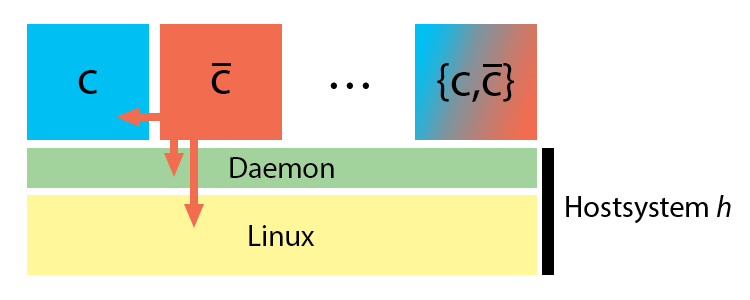
\includegraphics[width=0.8\textwidth]{./images/question_model2.png}
        \caption{Erweiterung des Systemmodells um ein Angreiferszenario (eigene Abbildung).}
        \label{fig:question_model2}
    \end{figure}

    %\begin{equation}
    %  C = \{c_1,c_2,\dotsc,c_i\;|\;0 < i < n \land C \neq \{\} \land i+j = N\}
    %\end{equation}
    %\begin{equation}
    %  C = \{c | 0 < i < n \land C \neq \{\} \land i+j = N\}
    %\end{equation}
    %\begin{equation}
    %  C' = \{c_1,c_2,\dotsc,c_j | 0 < j < n \land C' \neq \{\} \land i+j = N\}
    %\end{equation}
    %\begin{equation}
    %  \exists c \in M
    %\end{equation}
    %\begin{equation}
    %  \exists c' \in M
    %\end{equation}
    % TODO: iwas von hier aufnehmen? Oder sind obige zwei Formeln ausreichend? Sollten eig...

    Mit den Definitionen \ref{eq:subsets} und \ref{eq:unionset} wird ein Systemmodell erzeugt, das von mindestens zwei Containern in einem Hostsystem ausgeht. Mindestens ein Container \cvalid{} davon ist legitim und mindestens ein Container \cbroken{} ist kompromittiert.
    % TODO: Dieser Sachverhalt ist in \fig ... graphisch dargestellt.

    Damit bildet das Modell den Betrieb von Docker-Containern realitätsnah ab, da diese so konstruiert wurden, dass sie i.d.R. in einer Vielzahl parallel auf \(h\) laufen. Wie aus obiger Schlussfolgerung hervorgeht, muss angenommen werden, dass \(\overline{C}\) eine nicht-leere Menge ist, also mindestens ein Container \cbroken{} existiert, der Schadcode ausführt und die Sicherheitsziele von \(h\) und zu schützenden Containern in \(C\) verletzen kann. Beide Eigenschaften werden von diesem Systemmodell abgedeckt.

    % Ob das zugrundeliegende Image fehlerhaft bzw. manipuliert ist (Gefahr A), oder ein Container aktiv von einem Angreifer kontrolliert wird (Gefahr B), spielt für den Host keine Rolle. Der Host muss in der Lage sein, die Systemsicherheit aufrecht zu erhalten. Die Systemsicherheit umfasst hierbei den Schutz des Hosts sowie anderer Container.

    %Container c' aus dem Set C' ist in der Lage alle drei Sicherheitsziele zu verletzen. Man-in-the-Middle kann Vertraulichkeit verletzt werden, indem geheime Informationen abgefangen werden. Mit geheimen Informationen können unter Umständen Daten unrechtmäßig manipuliert werden, was die Integrität beeinflusst. Normale Programmflüsse können unterbrochen werden, was Beeinträchtigungen für die Verfügbarkeit mit sich zieht. Auch DoS-Attacken sind von c' aus möglich.

    %Einige der von c' geführten Angriffe sind nur durchführbar, wenn der Container im Besitz bestimmter Rechte ist. Die Privilegien, die ein Container standardmäßig besitzt, können fest definiert werden.

    %\emph{Privilege Escalation als extra Punkt aufführen? Ist eigtl kein direktes Sicherheitsziel. Eher im Punkt Gegenmaßnahmen aufführen....}

    Durch die Existenz von \cbroken{}, können die Sicherheitsziele der Vertraulichkeit, Integrität und Verfügbarkeit verletzt werden:

    \begin{itemize}
      \item \textbf{Vertraulichkeit}: \cbroken{} kann Aktionen ausführen, die unrechtmäßigen Zugriff auf Informationen von \(h\) und Container aus \(C\) ermöglichen. \\
      \textbf{Beispiele}: \acrshort{MITM}-Angriff, Lesen von Daten anderer Container
      \item \textbf{Integrität}: \cbroken{} kann Aktionen ausführen, die Daten von \(h\) und \(C\) manipulieren. \\
      \textbf{Beispiele}: Überschreiben oder Löschen von Daten anderer Container
      \item \textbf{Verfügbarkeit}: \cbroken{} kann Aktionen ausführen, um die von \(h\) vorgesehenen Mechanismen zur Aufrechterhaltung der Verfügbarkeit zu umgehen. Die Funktionstüchtigkeit von \(h\) und \(C\) kann dadurch beeinträchtigt werden. \\
      \textbf{Beispiele}: \acrshort{DoS}-Angriffe wie Erschöpfung von Hostsystemressourcen
    \end{itemize}

    %- Container compromise: compromise C k ∈ C by means of illegitimate
    %data access, Man-in-the-Middle (MitM) attacks or by affecting the control
    %flow of instructions executed in C k ∈ C.
    %- Denial of Service: disturb normal operation of the host or C k ∈ C.
    %- Privilege escalation: obtain a privilege not originally granted to a C j ∈ C.

  \section{Anforderungen an die Sicherheit von Containern}
    Aus den Annahmen und der Schlussfolgerung in Abschnitt \ref{questionEffects}, lässt sich eine allgemeine Sicherheitsanforderung formulieren:

    Von einem kompromittiertem Container \cbroken{}, darf der zu schützende Rest des Systems nicht betroffen sein. Die Sicherheitsziele der Vertraulichkeit, Integrität und Verfügbarkeit sollen für \(h\) und \(C\) gewahrt werden.

  \section{Theoretischer Lösungsansatz}
  \label{questionSolutionTheory}
    Die Strategie zur Erfüllung der definierten Sicherheitsanforderungen beruht unter Docker auf einem zweistufigen Ansatz:

    \begin{enumerate}[label=(\arabic*)]
      \item Angreifern soll es erschwert und bestenfalls unmöglich gemacht werden, aus der virtualisierten Umgebung eines \cbroken{} auszubrechen. Angreifer sollen nicht die Möglichkeit besitzen, die ursprünglich für \cbroken{} vorgesehenen Rechte zu erweitern.
      \item Falls es einem Angreifer dennoch gelingen sollte (1) zu verletzen, soll er durch weitere Zugriffskontrollen daran gehindert werden, Schaden in \(h\) und den zu schützenden Containern aus \(C\) anzurichten.
    \end{enumerate}

    Mithilfe der im nächsten Abschnitt aufgelisteten Mittel versucht Docker diese umzusetzen.

    %auf Modellebene:
    %1. + 2. setzen \emph{Defense in Depth} um.
    %2. setzt \emph{Principle of Least Privilege} um.

  \section{Umsetzung des Lösungsansatzes} % um Bedrohungspotential zu minimieren.
  \label{questionRealization}
    Zunächst lassen sich die möglichen Sicherheitsmechanismen in drei Arten unterteilen. Zur Einordnung der folgenden Kapitel sind diese kurz vorgestellt \cite[S.40ff.]{CISSP}\cite[S.23]{nist}:

    \begin{itemize}
      \item \textbf{Technische Kontrollen}: Umfasst alle hardware- und softwarebasierten Mechanismen, z.\,B. ein Zugriffsschutz unter Verwendung einer \acrshort{MAC-SEC}.
      \item \textbf{Administrative Kontrollen}: Enthält Managementkontrollen, die z.\,B. durch Konfigurationen, Entwicklung einer Sicherheitspolitik, Reduzierung der Fehleranfälligkeit durch Automatisierung und Sicherheitsschulungen des Personals umgesetzt werden.
      \item \textbf{Physische Kontrollen}: Beinhalten Mechanismen wie Sicherheitsschleusen, Schlösser und Wachpersonal. Obwohl ein Bezug zum Betrieb von Rechenzentren hergestellt werden kann, haben physische Kontrollen keine spezifische Relevanz für die containerbasierte Virtualisierung und sind aus diesem Grund an dieser Stelle nur zum Zweck der Vollständigkeit aufgeführt.
    \end{itemize}

    Docker hat als Softwareprodukt die Möglichkeit, direkt technische Kontrollen in die Codebasis einzubauen bzw. solche, die der Linux-Kernel implementiert, zu unterstützen. Auch verfolgt Docker administrative Sicherheitsansätze, die teilweise durch technische Mittel begünstigt werden.

    Die Umsetzung erfolgt mittels zweier Prinzipien, die am Anfang von Kapitel \ref{secLinux} vorgestellt sind.

  \section{Ziel der Arbeit}
    Gegenstand dieser Arbeit ist, die von Docker integrierten softwarebasierten und administrativen Maßnahmen zu analysieren.

    Im Rahmen der Arbeit werden die Sicherheitsmaßnahmen sowie deren Einsatz unter Docker vorgestellt. Die in diesem Kapitel erarbeiteten Annahmen und Schlussfolgerungen bilden dabei die Basis der Untersuchung. Die einzelnen Sicherheitsmerkmale sind dabei unabhängig von der Infrastruktur. Das bedeutet, dass sie bei einem lokalen Betrieb von Docker auf Computern von Entwicklern, bis hin zu Docker-Installationen in Cloud"=Infrastrukturen relevant sind.

    In dieser Arbeit wird auch betrachtet, welche Integrationsmöglichkeiten für Docker in Cloud"=Infrastrukturen existieren und welche speziellen Sicherheitskomponenten einsetzbar sind bzw. in welchem Umfang diese von externen Dienstleistern angeboten werden.

  %Docker setzt auf Software-Ebene überwiegend technische Kontrollen um, die kombiniert eine mehrschichtige \emph{Defense In Depth} bilden.
  % Docker als Softwareprodukt setzt überwiegend technische Kontrollen um (Kapitel 4). Aber begünstigt auch adminstrative Kontrollen (Kapitel 5).


  % Angewandt auf die Praxis: es muss universeller Ansatz gewählt werden, da jeder Kunde andere Sicherheitsanforderungen hat. Demnach können Schwachstellen, die die Vertraulichkeit, die Integrität oder Verfügbarkeit der Kundensoftware bedrohen, fatale Folgen für den Umsatz und die Reputation der Kunden und Betreiber von Rechenzentren ergeben.

  % Welche Sicherheitsmodelle und -mechanismen können eingesetzt werden, um Bedrohungspotential von aufgeführten Gefahrenquellen zu minimieren.

  % Darunter fallen mit Software realisierte Mechanismen zur Isolation, Ressourcenverwaltung und Zugriffskontrollen
  % Ziel der Arbeit: Halten diese CIA-Triade ein? Wie effektiv/weitrechend sind die eingesetzten modelle/mechanismen. Untersuchung der -modelle und -mechanismen in Bezug auf CIA-Traide.



  % Kommt man von Container auf Host-OS? Von Container auf anderen Container? ~etc.
  % 5-6 Sicherheitsziele erwähnen. Mit Forschungsfrage in Bezug bringen --> später bei Isolierung und Ressourcenverwaltung wieder aufgreifen

  % Allgemeiner Überblick zu Docker Security in \cite[S.3]{dockerSeec1}

  % (TODO): Schreiben, dass Container-Verschatelung bzw. Container in Hierarchien  ins Systemmodell absichtlich nicht aufgenommen wurden (was aber in FreeBSD jails moelgich ist).
  %   ^   (vgl. beide  \cite[S.4]{dockerSec2})

  % TODO: Sicherstellen, das Abgrenzung zu Netzwerkthemen da ist.

  %Das zentrale Konzept, auf dem alle Containertechnologien beruhen, ist das der Isolierung. Im Kontext von Containern kann die Isolierung definiert werden als Trennung zwischen Containern und einem Host, sowie die Trennung zwischen Containern \cite[S.1]{dockerSec2}.

  %Auf einem System mit Host und einem oder mehreren Containern, stellt sich zunächst die Frage welche Art und Richtung von Kommunikation zwischen diesen beiden Komponenten erlaubt und nicht erlaubt sein soll. Dadurch, dass der Docker-Daemon auf dem Host läuft und es dessen Aufgabe ist u.\,a. den Container-Lifecycle zu kontrollieren, braucht dieser Zugriff auf die Container. Verallgemeinert ist also die Kommunikation von Host zu Container erforderlich und damit erlaubt.

  %Was in einem Container passiert, ist zweitrangig, da der Container bei Fehlfunkionen jederzeit seitens des Hosts neu gestartet werden kann. Wichtig ist aber, dass der Container selbst von der Außenwelt, also dem Host und anderen Container, isoliert ist und seine Aufrufe gegen den Hostkernel streng limitiert sind und diese den Host nicht beeinträchtigen können.

  %Mehrere Sicherheitsfragen für Container-basierte Systeme sind in den folgenden Punkten formuliert. Sie beruhen auf der Annahme, dass ein Angreifer die Kontrolle über einen Container X übernommen hat und versucht, über diesen Schaden zu verursachen.

  %Situationen, in denen ein Angreifer bereits zu Beginn die Kontrolle über den Host hat, werden nicht betrachtet, da der Angreifer in dieser Lage bereits gewonnen hat und Container nach belieben manipulieren kann.

  %\begin{enumerate}[(1)]
  %  \item Ist es dem Angreifer möglich, seine in X erworbenen Rechte auf den Hosts zu erweitern, sodass er auf letzteren Root-Rechte erwirken kann? (Verletzte Sicherheitsziele: Vertraulichkeit, Authenzität, Integrität)
  %  \item Ist es dem Angreifer möglich, auf einen anderen Container Y des gleichen Hosts zuzugreifen? (Verletzte Sicherheitsziele: Vertraulichkeit, Authenzität, Integrität)
  %  \item Ist es dem Angreifer möglich, den Container oder Host auf eine Art und Weise zu beeinflussen, die den Betrieb anderer Container auf diesem oder entfernten Hosts beeinträchtigt? (Verletzte Schutzziele: Verfügbarkeit, Integrität) (Ressourcenverwaltung)
  %  \item Ist es dem Angreifer möglich, den Container X negativ zu beeinflussen oder ihn zum Absturz zu bringen? (Lifecyclemanagement des Docker-Hosts)
  %  \item Wie wird natürlichen Fehlfunktionen von Containern entgegengewirkt? (Lifecyclemanagement des Docker-Hosts)
          % Also wenn plötzlich Exception auftritt und Containeranwendung abstürzt.
  %  \item \emph{weitere Punkte?}
  %\end{enumerate}

  %Frage (1.) und (2.) zielen auf technischer Ebene auf die Isolation der Container ab. Eine Umformulierung in \glqq{}Sind Container ausreichend isoliert, um den Host zu schützen?\grqq{} ist möglich.

  %Wenn von der Netzwerkseite abgesehen wird, lässt sich das Szenario der Fragestellung (2.) auf das der Frage (1.) reduzieren, da der Zugriff auf andere Container nur über den lokalen Host möglich ist. Genauer gesagt ist der Zugriff auf andere Prozesse nur dann möglich, wenn Root-Rechte auf dem Host vorhanden sind. Die bereits generalisierten Sicherheitsfrage ist in (A.) unter Berücksichtigung dieses Punkts, erweitert

  %Die Fragen (3.), (4.) und (5.) teilen sich den Aspekt der Verfügbarkeit, der in Formulierung (B.) aufgegriffen wird.

  %Finale Umformulierungen und Generalisierungen:

  %\begin{enumerate}[(A)]
  %  \item Sind Container ausreichend isoliert, sodass ausgehend von Containern keine Root-Rechte auf dem Hostsystem erwirkt werden können?
  %  \item Kann der Betrieb von Containern negativ beeinflusst werden, sodass die Verfügbarkeit von Anwendungen darunter leidet?
  %  \item \emph{weitere Punkte?}
  %\end{enumerate}

  %, ob aus Containern ausgebrochen werden kann (1) und ob von einem Container X Zugriff auf einen Container Y auf dem gleichen Host möglich ist (2). Ist es unter der Annahme, dass ein Angreifer Zugriff auf einen Container erlangt, möglich, seine Rechte zu eskalieren und Root-Rechte auf dem Host zu erlangen? Diese Herausforderung spielt auch bei Frage (2) die entscheidene Rolle, da ein Zugriff auf andere Container erst mit einer Kompromitierung des Hosts möglichst ist. Aus diesem Grund genügt es, Frage (1) zu beantworten, da durch eine Antwort der selben auch die erweiterte Fragestellung (2) zufriedenstellend beantwortet werden kann.

  % Von entscheidender Bedeutung ist diese Frage, weil ihre Beantwortung die Existenzgrundlage für Container und damit auch Docker bildet. Gäbe es keine Methodeberuht. Wäre die Frage im Produkt Docker nicht beantwortet,

  %\emph{ALT:}


  % Technische Sicherheit
  %Um Frage (1.) zu beantworten, wird im ersten Hauptkapitel die intrinsische Sicherheit von Docker untersucht. Damit ist eine Reihe von Sicherheitsfeatures des Linux Kernels gemeint, die u.\,a. Docker nutzt, um nach Aussage von \emph{Docker} sichere Container zu ermöglichen. Genauer werden Mechanismen zur Isolation, Ressourcen- und Zugriffsverwaltung betrachtet, da sie direkt mit den erwünschten Sicherheitszielen aus Kapitel \ref{introSecGoals} in Bezug stehen.

  %Des Weiteren stellt sich die Frage, ob die Arbeit mit Docker und seinen Containern sicher ist. Wie in der \hyperref[dockerIntro]{Einführung zu Docker} beschrieben, stellt Docker zusammen mit anderen Anbietern einen Workflow und eine Palette an Tools zur Verfügung, die die Arbeit mit Containern erleichtern sollen. Wie diese Tools zur Sicherheit bzw. Angreifbarkeit von Docker-Systemen beitragen, wird im Kontext von den Sicherheitszielen betrachtet.
  % Technische und administrative Sicherheit

  %Nicht betrachtet werden die Sicherheitsrisiken, die sich durch den Betrieb eines Rechnernetzwerks ergeben, in dem Docker-Knoten existieren. Sicherheit aus Sicht der Netzwerktechnik und den verschiedenen \acrshort{OSI}-Schichten ist nicht Gegenstand der Untersuchung.

  % TODO: einarbeiten: Siehe \cite[S.3]{virtVSContainer} ... rechts oben ..

  % Da Images aud dem Docker Hub malicious sein koennen ,,,, arbitray code ausgefuehrt wird ...
  % kann auch ein Container, der diesen Code ausfuehrt, nicht vertraut werden /--> kann malicious werden (boesartig, boese absichten verfolgen)

\end{document}
